%%%%%%%%%%%%%%%%%%%%%%%%%%%%%%%%%%%%%%%%%%%%%%%%%%%%%%%%%%
%
% Doctoral Thesis Template @ The University of Manchester
% LaTeX Chapter Template
% Version 1 (23/07/2020)
% Joe Crone
%
% This template is based on:
% The University of Manchester, Presentation of Thesis Policy
% Research Office Graduate Education Team
% June 2017
% http://www.regulations.manchester.ac.uk/pgr-presentation-theses/
%
%%%%%%%%%%%%%%%%%%%%%%%%%%%%%%%%%%%%%%%%%%%%%%%%%%%%%%%%%%
\documentclass[../main.tex]{subfiles}
\begin{document}

% Title
%--------------------------------------------------------
\chapter{Introduction}
\label{Introduction} % to reference use \ref{ChapterTemplate}

Energy recovery Linacs (ERLs) are ideal drivers of inverse Compton scattering sources (ICS) due to the combination of linac quality beams and high repetition rate, allowing production of a tunable high-flux, narrowband scattered photon beam. The pioneering demonstration of multi-pass energy recovery in a superconducting RF (SRF) linac with FFAG return loop at the Cornell University Brookhaven National Laboratory Energy Recovery Linac Test Accelerator (CBETA) \cite{hoffstaetter2017cbeta} reveals a route to high energy electron beams for ERL driven ICS production of X-rays and $\gamma$-rays.

Due to a $E_{\gamma} \propto 4\gamma^{2}$ scattered photon energy $E_{\gamma}$ dependence, where $\gamma$ is the Lorentz factor, ICS is the prime candidate for production of high energy photons above photon energies available at conventional X-ray production facilities such as Free Electron Lasers (FEL)($E_{\gamma} <$~25~keV \cite{schneidmiller2011photon}) and the largest synchrotrons ($E_{\gamma} <$~500~keV) \textcolor{blue}{***Needs citation***}. Therefore, inverse Compton scattering sources are also the eminent method for high-flux production of $\gamma$-rays ($E_{\gamma} \sim$~1~MeV), which could support applications like nuclear resonance fluorescence (NRF) and nuclear photonics. ICS sources can be optimised to produce photons in smaller natural bandwidth than synchrotron radiation, alleviating the need for monochromators which inherently deplete the flux of the source. 

Experience gained this year from participating in CBETA commissioning and designing an X-ray ICS utilizing CBETA will ultimately motivate design choices and optimisations for an inverse Compton source operating on the posited Daresbury Industrial Accelerator for Nuclear Physics Applications (DIANA) ERL. The design values for the CBETA ICS are 4.64$\times 10^{8}$~ph/s in a 0.5\% bandwidth \textcolor{blue}{***Check flux figure hasn't changed***}up to a maximum photon energy of 401.4~keV. In comparison, the DIANA $\gamma$-ray source will be capable of producing $\sim 10^{11}$~ph/s in a 0.5\% bandwidth with scattered photon energies in the 1-20~MeV range, competitive with the flagship ELI-NP-GBS \cite{adriani2014technical} linac based inverse Compton scattering source. 

\section{Energy Recovery Linacs}

The energy recovery linac is a re-circulated linac concept, invented by M. Tigner in 1965 \cite{tigner1965possible} to improve the efficiency of particle colliders, where upon re-circulation the particle beam energy post-interaction is recovered in the same RF cavities that provided the initial acceleration. The recovered energy can then be applied to accelerate a following electron bunch, without additional application of RF power, to improve the efficiency of particle accelerators. Another benefit is that the particle beam is decelerated, and the dumped power of the particle beam as well as its energy are reduced. A further, more detailed explanation of an energy recovery linac is shown in Chapter~\ref{Energy_Recovery_Linac_Design}.

The ERL concept was first demonstrated in the superconducting accelerator driven Free Electron Laser (SCA/FEL) \cite{smith1987development} -- the first superconducting RF ERL. The SCA/FEL was capable of producing a 93~\si{\mega\electronvolt} electron bunch with 5~\si{\milli\meter}--\si{\milli\radian} emittance, a 5~\si{\pico\second} bunch length and 150~\si{\micro\ampere} average beam current. As well as the first demonstration of an ERL, the SCA/FEL demonstrated the efficacy of an ERL as a driver of a light source by demonstrating a UV FEL operating at $\lambda = 0.2$~\si{\micro\meter}.

ERLs have also been demonstrated using normal conducting RF (NCRF) cavities, such as the Chalk River Reflexotron \cite{schriber1977experimental} and the Los Alamos FEL \cite{feldman1987energy}, however these are typically low electron energy machines $E_{e} < 30$~\si{\mega\electronvolt} (Reflexotron 25~\si{\mega\electronvolt}, Los Alamos FEL 23.5~\si{\mega\electronvolt}). Normal conducting ERLs are limited because NCRF cavities are susceptible to cavity losses and RF transport losses \cite{adolphsen2022european} in comparison to SRF cavities, therefore the increase in efficiency -- re-use of RF power -- from energy recovery is less beneficial because the RF power is dissipated. Therefore, for high current (10's~\si{\milli\ampere}) and beyond moderate energies ($E_{e} > 100$~\si{\mega\electron}) with efficient use of RF acceleration, the development of superconducting RF ERLs is required.

All ERLs discussed so far were demonstrated using pulses or trains of electron bunches, however by using continuous wave ERLs the average beam current of the ERL can be improved. Continuous wave ERL operation was first demonstrated \cite{neil2000sustained} by the IR FEL demo \cite{benson1999first,neil2000sustained} at Jefferson Laboratory (J-Lab), where a single turn ERL was used to drive an infrared (IR) FEL. The J-Lab IR FEL demo produced an average beam current of 4.8~\si{\milli\ampere} with a 48~\si{\mega\electronvolt} producing a peak current of 60~\si{\ampere} for production of $\lambda =$ 3--5.3~\si{\micro\meter} infrared radiation with an average power of 1.72~\si{\kilo\watt}. Subsequently, with experience operating the IR FEL demo, an upgraded J-Lab IR FEL was designed \cite{benson2002have} and built \cite{behre2004first} with an upgraded higher average beam current injector, improved beam dynamics design and improved FEL design. The J-Lab IR FEL upgrade produced a maximal average beam current of 9.1~\si{\milli\ampere} -- a record for SRF ERLs -- with a 160~\si{\mega\electonvolt} electron bunch, a total beam power of 1.46~\si{\mega\watt} \cite{neil2006jlab}. The IR Upgrade ERL operated near 1.5~\si{\mega\watt} of electron beam power with only around 300~\si{\kilo\watt} of installed RF power \cite{adolphsen2022european}, which demonstrates the ability of the ERL concept to produce high-power light sources whilst reducing the required RF power.  

Another ERL has subsequently been developed at J-Lab -- the Continuous Electron Beam Accelerator Facility (CEBAF) \cite{bogacz2003cebaf,tennant2003beam} -- which was originally designed as a re-circulated linac but demonstrated single turn energy recovery in 2003. CEBAF demonstrated energy recovery of a 1.02~\si{\giga\electronvolt} electron beam, the highest energy electron beam energy recovered worldwide, with a normalised transverse emittance of $\epsilon_{nx} \left(\epsilon_{ny}\right) = 2.39 \left(2.06\right)$~\si{\milli\meter}--\si{\milli\radian} \cite{tennant2003beam}. ERLs within the \si{\giga\electronvolt}-scale have uses as $\gamma$-ray factories \cite{budker2021expanding}, utilising ICS sources, and particle collider applications \cite{agostini2021large} for high energy particle physics. 

Since demonstration of the J-Lab FEL, the high current frontier of 10's~\si{\milli\ampere} has been pursued by the compact ERL (cERL) at KEK \cite{akagi2016narrow}, where demonstration of a 10~\si{\milli\ampere} average beam current is planned with 100\% energy recovery efficiency \cite{adolphsen2022european}. Currently, an average beam current of 1~\si{\milli\ampere} has been achieved at cERL \cite{obina20191} with an energy recovery efficiency of $100\pm 0.5$\%. Light sources other than FEL have been applied to ERLs such as the 
ICS sources applied to the ALICE ERL at Daresbury Laboratory \cite{priebe2008inverse,priebe2010first} and the ICS source applied to cERL \cite{akagi2016narrow}. The ICS sources take advantage of the high electron beam brightness delivered by an ERL like FELs. However, ICS source demonstrations upon ERLs have been limited to low energies (ALICE $E_{e}=30$~\si{\mega\electonvolt}, cERL  $E_{e}=20$~\si{\mega\electronvolt}) and low current $I < 1$~\si{\milli\ampere}, so only x-ray photons at low fluxes can be produced. 

The Novosibirsk Recuperator NCRF ERL driven FEL is the first demonstrated multi-turn ERL \cite{gavrilov2007status} in which the electron bunch is accelerated for multiple passes before deceleration for multiple passes.  Multi-turn ERLs are advantageous because the electron beam can be repetitively accelerated, allowing for a larger maximum electron energy for the same RF acceleration section as a single turn ERL. The highest average electron beam current in an ERL demonstrated at 30~\si{\milli\ampere} has also been achieved in the Novosibirsk FEL \cite{gavrilov2007status}. A recent upgrade of the RF gun has demonstrated up to 100~\si{\milli\ampere} average beam current \cite{matveev2020simulation}, which could provide an average beam current in an NCRF ERL an order of magnitude larger than the 9.1~\si{\milli\ampere} \cite{neil2006jlab} demonstrated for SRF ERLs.  

Multi-turn ERLs have been demonstrated with SRF accelerating structures firstly by the CBETA ERL \cite{bartnik2020cbeta} and then recently by S-DALINAC ERL \cite{adolphsen2022european}. For multi-turn energy recovery operation up to 81.8\% of the electron bunch energy was recovered in S-DALINAC, with a maximum beam current of 8~\si{\micro\ampere} -- the highest energy recovery efficiency demonstrated for a multi-turn SRF ERL. Both accelerators, CBETA \cite{gulliford2021measurement} and S-DALINAC
\cite{steinhorst2021rf} were first operated as single turn ERLs with 99.4\% and 90.1\% energy recovery efficiency respectively. However, currently only low average beam currents have been demonstrated by multi-turn ERLs, with a maximum 8~\si{\micro\ampere} average beam current. CBETA commissioning is explained in more detail in Section~\ref{sec:CBETA_commissioning}.

A comprehensive plot of the electron beam energy and average beam current achieved by various ERL projects is shown in Fig.~\ref{fig:ERL_Landscape}, which is also indicative of the average electron beam power of the ERL. Currently a maximum electron beam power demonstrated in an ERL is 1.46~\si{\mega\electronvolt} using the J-Lab upgraded FEL \cite{neil2006jlab}, and the maximum electron beam energy demonstrated in an ERL is the $\sim1$~\si{\giga\electronvolt} energy recovery demonstration using CEBAF \cite{bogacz2003cebaf,tennant2003beam}. However, several projects are in development seeking to demonstrate ERLs with higher average current, higher electron bunch energies and multi-turn designs, such as PERLE \cite{angal2018perle}, bERLinPro \cite{kuske2012conceptual} and ER@CEBAF \cite{meot2016er}.

\begin{figure}[!h]
\centering
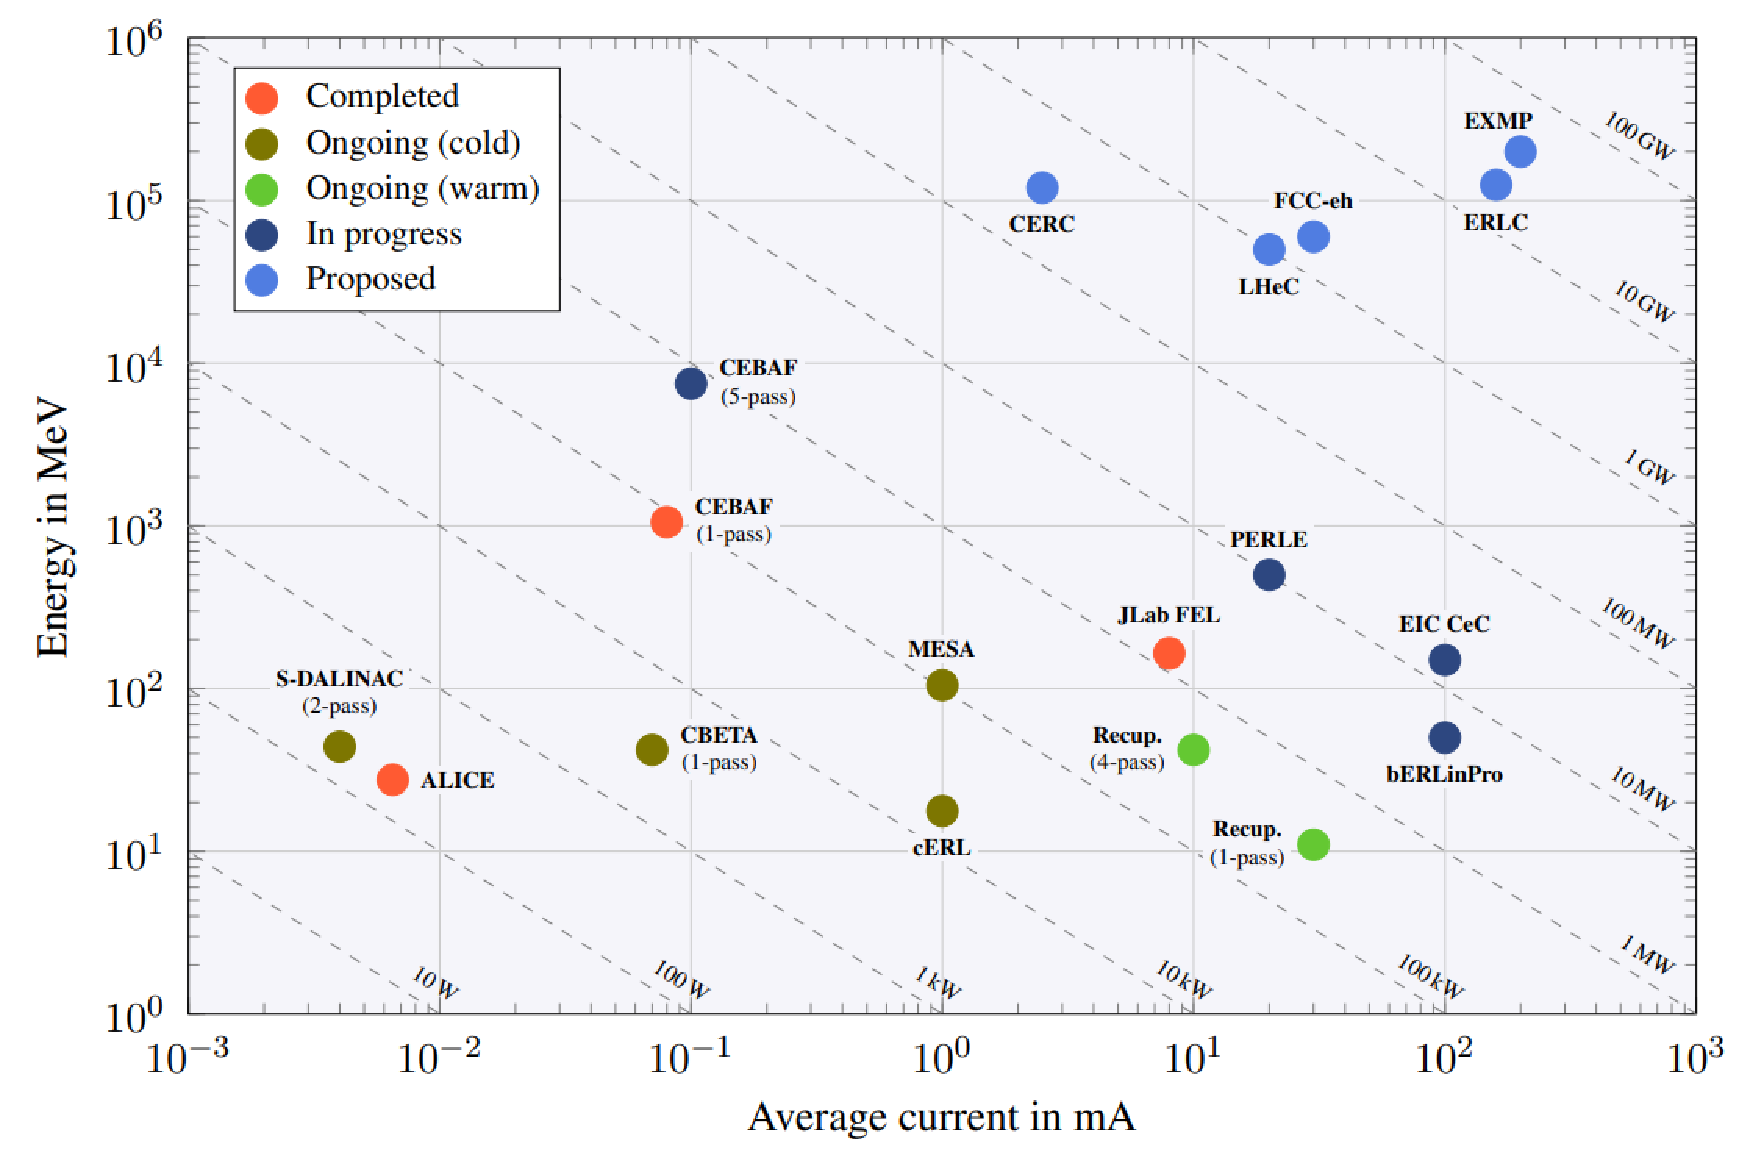
\includegraphics[width=0.9\textwidth]{Figures/CBETA_Multi-Pass_Commissioning/Tennant_ERL_Landscape.pdf}
\caption{The landscape of legacy, ongoing and proposed ERL projects plotted as a function of maximum electron beam energy and average beam current. Gridlines denote the average electron beam power. Reproduced from the European Strategy for Particle Physics
Accelerator R&D Roadmap \cite{adolphsen2022european}.}
\label{fig:ERL_Landscape}
\end{figure}

The bERLinPro ERL is a single turn ERL which aims to demonstrate high current operation of an ERL with a maximum average beam current of 100~\si{\milli\ampere} at 50~\si{\mega\electronvolt} electron beam energy \cite{kuske2012conceptual,neumann2018berlinpro}. A normalised transverse emittance of 1~\si{\milli\meter}--\si{\milli\radian} emittance with a 2~\si{\pico\second} bunch duration is projected, which would be the highest brightness electron bunch produced in an ERL. However, commissioning of the bERLinPro ERL has been stalled by damage to the main linac cryomodule \cite{neumann2018berlinpro}. Many obstacles to high average current operation in ERLs exist, as explained in Section~\ref{sec:high_current_ERL}, such as coherent synchrotron radiation production, beam breakup instability and beam halo -- the latter two are an active area of study for bERLinPro \cite{neumann2012status,hwang2019first}. High current operation is necessary for light source operation of ERLs, such as ICS sources and FELs.  

The ER@CEBAF experiment aims to extend the operation of electron ERL to high electron energy operation with a maximum electron energy of 7.5~\si{\giga\electronvolt} \cite{bogacz2016er,meot2016er}. In addition, the ER@CEBAF ERL is a 5-turn design -- the most turn design of any ERL -- with the potential to demonstrate the many-turn route to \si{\giga\electronvolt} electron energy ERLs. Attaining high electron energies within a compact footprint is the main advantage of a multi-turn ERL, therefore ER@CEBAF is a necessary demonstrator for future collider projects such as the LHeC electron--positron collider \cite{valloni2013strawman,bruning2019exploring,holzer2021accelerator}. Impact of the synchrotron radiation losses of a 7.5~\si{\giga\electronvolt} electron beam energy, as in the ER@CEBAF ERL design, upon the beam dynamics of an ERL would be challenging therefore the ER@CEBAF project could allow for study of synchrotron losses upon momentum acceptance in the single transport optics \cite{adolphsen2022european}.  

PERLE: powerful energy recovery linac for experiments is the highest average electron beam power ongoing ERL project with an electron beam energy of 500~\si{\mega\electronvolt} and average electron beam current of 20~\si{\mill\ampere} -- an average electron beam power of 10~\si{\milli\watt} \cite{angal2018perle,bogacz2021perle}. PERLE -- a three turn common transport ERL -- is designed to provide a moderate energy, moderate current demonstration toward the proposed LHeC project \cite{valloni2013strawman,bruning2019exploring,holzer2021accelerator}. Important ERL topics studied at PERLE will include handling a high average beam current, low electron beam energy spread and emittance at an IP and CW operation \cite{adolphsen2022european} necessary toward future colliders. To achieve a high average electron beam current PERLE utilises a high bunch charge of 500~\si{\pico\coulomb} \cite{}, a factor $\sim3$ higher than previously demonstrated in an SRF ERL at the upgraded J-Lab FEL \cite{neil2006jlab}. The PERLE ERL is designed with an integrated final focus system which, with 500~\si{\mega\electronvolt} electron bunches, makes PERLE an ideal driver of a ICS source \cite{adolphsen2022european}; using an IR laser (Nd:YAG $\lambda=1064~\si{\nano\meter}$) PERLE is capable of generating up to 4.45~\si{\mega\electronvolt} $\gamma$-rays.      

Multi-turn ERLs in particular are a good choice for design of a light source because, as previously demonstrated, multi-turn ERLs can deliver high average electron beam power (\si{\mega\watt}-scale) with small emittances ($\epsilon_{n} < 1$~\si{\milli\meter}) and short bunch lengths (\si{\pico\second}-scale) which constitute high brightness electron beams. In addition, multiple re-circulations allows for higher energy electron beams necessary for small wavelength photon generation to be produced in a compact footprint, without an expensive high power accelerating section. Hence, multi-turn ERLs are investigated as drivers of light sources within this thesis.    

\section{Synchrotron Radiation Production}

% first demonstration + description of process
Synchrotron radiation was first observed experimentally in 1947 at the GE synchrotron, New York, USA \cite{elder1948radiation} and the first classical description of synchrotron radiation was published by Schwinger in 1949 \cite{schwinger1949classical}, after experimental verification using the GE synchrotron. Synchrotron radiation is produced when the trajectory of a relativistic particle beam is curved by an applied electromagnetic field, such as a dipole magnetic field, and emits radiation. The particle beam is subject to a Lorentz force due to the applied magnetic field causing an acceleration and subsequently the emission of radiation. Viewed in the reference frame of the particle beam, the emission pattern of this radiation is the familiar dipole radiation pattern -- a toroidal radiation pattern with maximum intensity perpendicular to the applied field (parallel to the velocity of the electron). However, if the particle beam has an ultra-relativistic velocity i.e the Lorentz speed factor is near unity ($\beta\sim1$), then in the laboratory frame the toroid is strongly deformed because of the Doppler effect and is elongated into a cone with axis parallel to the velocity of the particle \cite{ternov1995synchrotron}. Emission intensity in both the relativistic and non-relativistic case is shown in Fig.~\ref{fig:synchrotron_radiation_diagram}. Synchrotron radiation within an accelerator context is described in further detail in Section~\ref{sec:synchrotron_facility_comparison}.

\begin{figure}[!h]
\centering
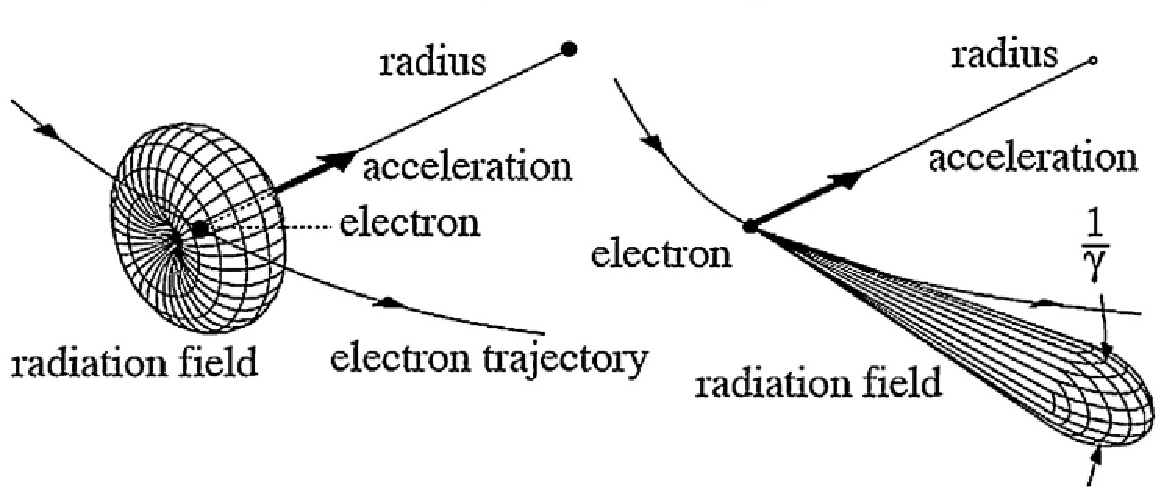
\includegraphics[width=0.8\textwidth]{Figures/Introduction/Synchrotron_Radiation_Diagram.pdf}
\caption{Diagram of the emitted synchrotron radiation fields produced by a charge moving at relativistic velocity $v$ ($\beta\sim 1$)subject to a constant dipole magnetic field causing the electrons to traverse a curved trajectory. Reproduced and modified from \cite{eberhardt2015synchrotron}. Left: Toroidal field observed in the electron reference frame. Right: Elongated cone field, with opening angle $\theta = 1/\gamma$, observed in the laboratory frame.}
\label{fig:synchrotron_radiation_diagram}
\end{figure}
% why is it useful in comparsion to other sources
Synchrotron radiation is useful experimentally because it is significantly higher flux than x-ray Bremsstrahlung generation, for example the SPring-8 synchrotron radiation source has a maximum average brilliance of $10^{20}$~ph/\si{\second} \si{\milli\meter}$^{2}$--\si{\milli\radian}$^{2}$ 0.1\% BW \cite{spring8beamlines} whereas $10^{10}$~ph/\si{\second} \si{\milli\meter}$^{2}$--\si{\milli\radian}$^{2}$ 0.1\% BW is possible from modern bremsstrahlung based x-ray tubes \cite{behling2018diagnostic}. Short duration radiation is required for investigation of temporally varying phenomena such as functional processes in structural biology which occur on picosecond to nano-second scales \cite{burnett2020uk}, with  10's~\si{\pico\second} x-ray pulses demonstrated for synchrotron radiation production -- for example the 32~\si{\pico\second} x-ray pulse duration of SPring-8 measured at 14~\si{\kilo\electronvolt}. Comparably, a 2~\si{\milli\second} x-ray pulse duration is readily achieved x-ray tubes \cite{behling2018diagnostic}. Synchrotron radiation wavelengths may also be tuned via variation of the magnet strength or, for undulator radiation, via variation of the undulator period. Emission angles $\theta$ of synchrotron radiation are also small with radiation produced in a cone of $1/\gamma$; for an 8~\si{\giga\electronvolt} electron beam the opening angle of the radiation is $\sim 64$~\si{\micro\radian}, producing a small radiation spot size on-sample.        

% First dedicated experiments (2nd Gen)
As the utility of the produced radiation was understood, numerous experiments were conducted parasitically such as the x-ray spectroscopic measurements of Berylium K-edges with the Cornell 320~\si{\mega\electronvolt} synchrotron \cite{johnston1954absorption}. The first dedicated accelerator for production of synchrotron radiation, known as a 2nd generation light source, was Tantalus I \cite{rowe1973tantalus}, first operated in 1968. Similar facilities were constructed across Europe in the following 10--15 years, with increased electron energy for access to higher photon energies, such as the worlds first high energy Synchrotron Radiation Source (SRS) at Daresbury \cite{munro2019fifty,robinson1981experiments}. 

% Monochromation + why we want brilliance not flux
High brilliance is desired by many synchrotron facility users, such as those conducting spectroscopy and crystallogrphy experiments, because these experiments monochromate the produced synchrotron radiation pulse. Monochromation involves using Bragg diffraction from perfect (defectless) crystals to select a narrow bandwidth (small energy spread in the produced radiation) of the synchrotron radiation pulse. Diffraction angle is wavelength (energy) dependent therefore a narrow bandwidth can be selected via optics post monochromation. Further details on monochromation of synchrotron radiation are explained by Caciuffo et al \cite{caciuffo1987monochromators}. A small radiation spot size and angular divergence upon the monochromator is required so the radiation pulse impinges on the monochromator with similar angle irrespective of position in the radiation pulse. Therefore, maximising the synchrotron radiation flux to the monochromator -- dependent on radiation pulse spot size and divergence -- is ideal for synchrotron radiation users, and brilliance is a measure of this. Brilliance of a radiation beam can only be improved via improvements in the electron beam -- the source of the radiation -- which is readily achieved by decreasing the emittance of the electron beam. Therefore, storage rings were designed to produce lower emittance electron beams by using optics solutions such as the double bend achromat design proposed by Chasman and Green \cite{chasman1975preliminary}.          

% 3rd Generation light sources
% undulators + wigglers 
% GeV scale km circumference machines
Synchrotron radiation facilities were further advance by the emergence of lower emittance designs, higher energies and the advent of insertion devices such as wigglers and undulators which are termed 3rd generation light sources. Undulators consist of a straight accelerator beamline populated by permanent magnets of varying polarity. In their simplest and most common form, the planar undulator, this consists of two perpendicular periodic series of alternating polarity vertical dipole magnets, as shown in Fig.~\ref{fig:planar_undulator}, which causes the electron bunch to travel on a sinusoidal oscillatory trajectory with synchrotron radiation produced in each bend. The radiation produced by each subsequent bend, or period, of the undulator overlaps spatially creating a high brilliance fundamental radiation peak and, due to the short bend, is monochromatic. Wigglers operate via a similar principle, however these use higher field magnets with fewer periods resulting in a high flux continuous spectrum of radiation which can achieve smaller wavelengths (higher energies). 

\begin{figure}[!h]
\centering
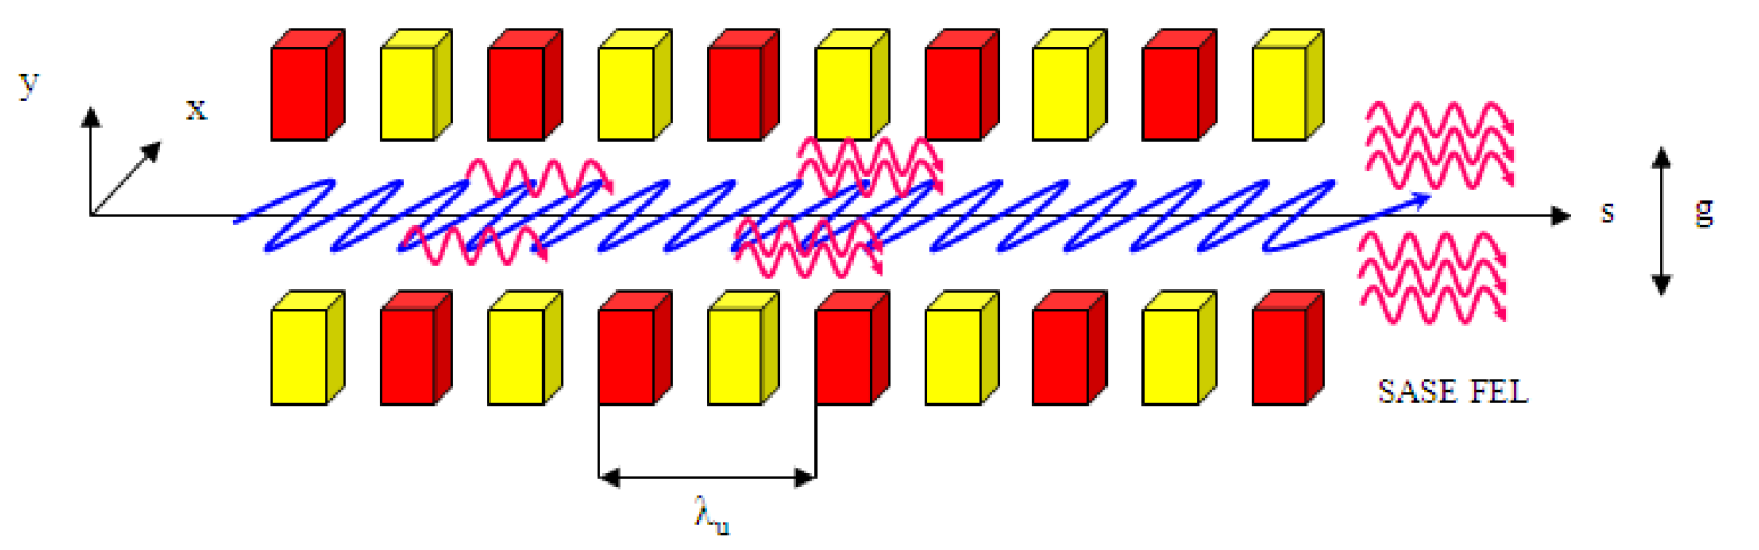
\includegraphics[width=\textwidth]{Figures/Introduction/Planar_Undulator.pdf}
\caption{Diagram of a planar undulator with magnet gap $g$ and undulator period $\lambda_{u}$ with alternating polarity magnets (red, yellow). The electrons to follow an oscillatory trajectory (blue) within the planar undulator field, which causes the emission of synchrotron radiation (red). Throughout the undulator the self-interaction of the electron beam with the synchrotron radiation produces a microbunched electron beam and coherent radiation. Reproduced from Kentenoglu and Yavas \cite{ketenoglu2010asynchronously}.}
\label{fig:planar_undulator}
\end{figure}

The first undulator, was demonstrated in 1953 using a linac at Stanford university \cite{motz1953experiments}, then subsequently demonstrated in straight sections of the LPI RAS synchrotron light source in 1977 \cite{bessonov2010light}.  However as undulators require a large number of magnets these could not be practically implemented until the design of permanent magnet undulators by Hallbach et al \cite{halbach1983permanent}. Undulators were then widely utilised in synchrotron sources. Similarly, wigglers were demonstrated in 1979 \cite{berndt1979initial} but became favoured devices for synchrotron production at the shortest wavelengths through use of high field superconducting magnets. For example, a 10~\si{\Tesla} wiggler was demonstrated with an 8~\si{\giga\electronvolt} electron beam at SPring-8, generating \si{\mega\electronvolt}-scale $\gamma$-rays \cite{soutome2003generation}.    

% Free electron lasers
An undulator alone produces incoherent radiation, where different electrons in the bunch radiate at varying times. Consequently, the radiation pulse duration from an undulator can be large. However, coherent radiation -- where radiation is produced simultaneously from and electron bunch -- can be produced from an undulator when the longitudinal distribution of the electron beam is bunched at the wavelength of the produced radiation, however achieving this longitudinal distribution can be challenging. In an FEL the power of undulator radiation is increased via coherent enhancement, where constructive interference occurs from consecutively emitted undulator radiation. The power of a free electron laser therefore increases proportionally to $N^{2}$, where $N$ is the number of electrons traversing the undulator. Therefore, a free electron laser provides a monochromatic, high power temporally and spatially coherent radiation pulse to users.  

The required electron beam longitudinal distribution for free electron lasing can be achieved in numerous ways, but is typically achieved by self amplification by spontaneous emission (SASE) or seeding approaches. In SASE operation, self-interaction between the electron bunch and the generated undulator radiation causes energy exchange between the radiation field and the electron bunch which, with many electron bunch--radiation filed interactions, drives microbunching of the electron bunch. The microbunched electron beam has the required longitudinal distribution and therefore coherent emission occurs. However, temporal coherence is compromised because the SASE process is started radomly from `shot noise' i.e the microbunching is generated by the incoherent undulator radiation, though this can be overcome via monochromating the radiation pulse before it is used to seed lasing in a process known as self seeding, such as the diamond monochromator used for self-seeding the LCLS x-ray FEL \cite{emma2010first
}. Self-interaction of the undulator radiation with the electron bunch can be achieved via use of a small undulator and a series of mirrors, known as an optical cavity, to circulate the produced radiation for interaction or by use of a long undulator where radiation produced from the $n+1$\textit{th} interacted electron bunch interacts with the $n$\textit{th} electron bunch. A diagram of a long planar undulator used for SASE FEL generation is shown in Fig.~\ref{fig:planar_undulator}. % this is SASE - SASE with optical mirrors too (long undulator or optical mirrors) % mention starting from noise? - worse temporal coherence?

% Seeding - limited by available seeds i.e no x-ray seeding possible (need initial coherent source)
Self-interaction can be seeded, by using an initial, often low power, external source of coherent radiation such as a conventional laser which initially microbunches the electron beam. A coherent seed means the produced radiation is also coherent, and avoids the temporal coherence issues associated with SASE methods. Higher harmonics of the initial seeding laser may be used in order to generate higher wavelength radiation. However, seeded FELs are fundamentally limited by a lack of coherent sources beyond the \si{\nano\meter}-scale. The first free electron laser was demonstrated at Stanford University in by Deacon et al \cite{deacon1977first} in 1977, with infrared lasing (coherent photon production) at a wavelength of $\lambda = 3.41$~\si{\micro\meter} and 7~\si{\kilo\watt} peak power. The initial Stanford FEL experiment was an example of a seeded FEL. The lowest wavelength seeded FEL demonstrated to date is the FERMI@ELETTRA FEL \cite{allaria2012highly} with a minimum wavelength of $\sim10$~\si{\nano\meter}; seeded FELs are yet to probe the x-ray regime. The first x-ray FEL LCLS was first demonstrated in 2010 at SLAC, with a minimum wavelength of 1.2~\si{\angstrom}, a sub pico-second pulse duration (500--10~\si{\femto\second}), a 0.2--0.5\% FWHM bandwidth and up to 40~\si{\giga\watt} peak power \cite{emma2010first}.

The peak brilliance -- a measure of the photons produced per pulse duration per unit area in phase space within a small 0.1\% energy spread (bandwidth) (see Chapter~\ref{Photon_Production_by_Inverse_Compton_Scattering}) -- of a series of world-leading light sources are shown in Fig.~\ref{fig:light_source_tuning_curves}. Brilliance is often termed brightness, both are identical quantities, however the convention of brightness for electrons and brilliance for photons is used in this thesis. 

\begin{figure}[!h]
\centering
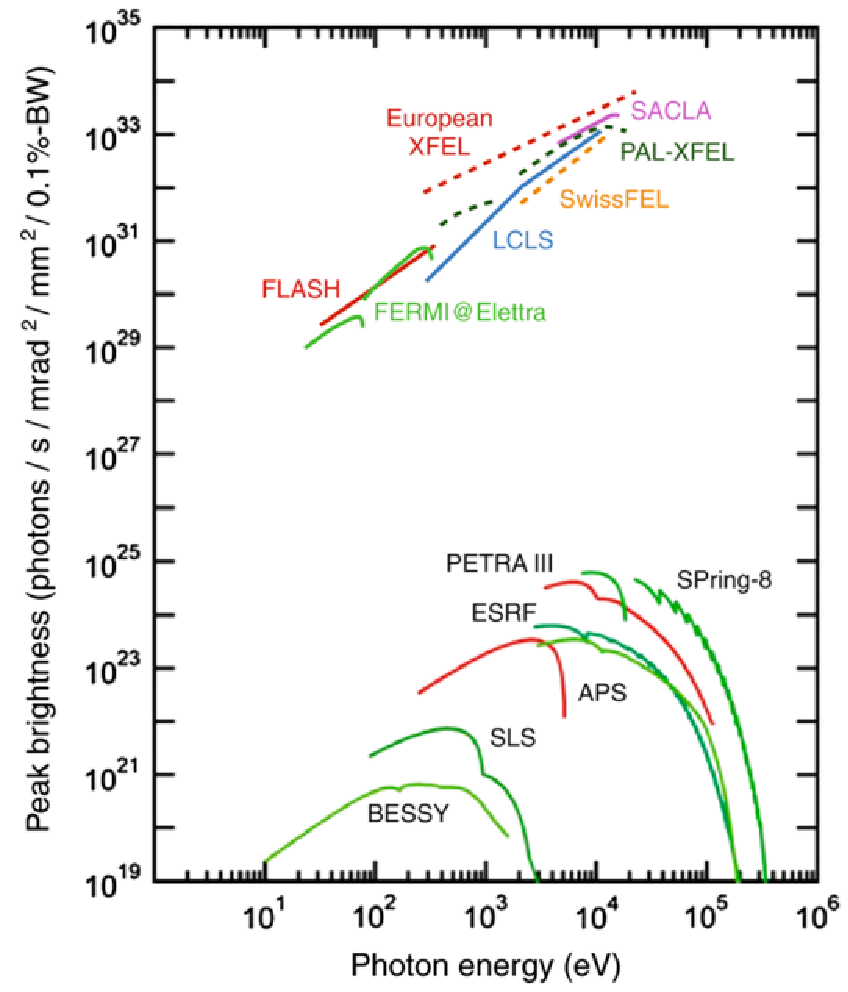
\includegraphics[width=0.6\textwidth]{Figures/Introduction/Light_Source_Brilliance_Energy.pdf}
\caption{Peak brilliance--photon energy tuning curves of a collection of existing x-ray light source facilities, showing both free electron lasers and synchrotron light sources \cite{geloni2017physics}. Note that brilliance is termed brightness here, whilst the two are identical brightness is reserved for discussion of electrons in this thesis.}
\label{fig:light_source_tuning_curves}
\end{figure}

Ultimately, as demonstrated in Chapter~\ref{CBETA_Inverse_Compton_Scattering_Source_Design}, practical considerations limit synchrotron radiation facilities and free electron lasers to x-ray production. For development of a $\gamma$-ray source, methods based on synchrotron or undulator radiation fail to produce the \si{\mega\electronvolt}-scale photons desired by nuclear physics experiments \cite{budker2021expanding}. However, synchrotron radiation facilities and FELs are the dominant radiation production methods in the x-ray regime and below, with unparalleled photon flux and brilliance.  

\section{Bremsstrahlung Radiation Production}
\label{sec:bremsstrahlung}
% Hywels lecture notes give a good brief overview of Brem (in the chapter comments directory) + have the review he gave me
% Duane - Hunt law
% Continuous spectrum - hard to monochromate - why no gamma monochromators?
% High Z good, why? High field for breaking


\section{Inverse Compton Scattering Sources}
% electron photon collider
% laser undulator
% limitations of the compton cross section - flux
An alternative radiation production mechanism to the more commonplace synchrotron sources and free electron laser facilities is to use the inverse Compton scattering process. The inverse Compton scattering process was first considered by Feenberg and Primakoff \cite{feenberg1948interaction} as a mechanism whereby cosmic rays are reduced in energy as they propagate throughout the universe. The cosmic rays -- relativistic charged particles -- interact with starlight to emit smaller wavelength radiation, with the concurrent reduction in energy of the relativistic charged particle. The inverse Compton process is opposite to Compton scattering \cite{compton1923quantum}, where a non-relativistic particle interacts with a photon lengthening the incident photon wavelength and increasing the energy of the incident particle. An extended discussion of Compton and inverse Compton scattering is found in Section~\ref{sec:electron_photon_interactions}. 

Savedoff \cite{savedoff1959crab} and later Felten and Morrison \cite{felten1963recoil} suggested the use of inverse Compton scattering as a radiation production method, specifically for $\gamma$-rays, which are difficult to obtain due to their inherent high energy. Radiation sources using the principle of inverse Compton scattering can be considered as electron--photon colliders or as laser undulator devices, as shown diagramatically in Fig.~\ref{fig:}. The electron--photon collider model involves a collision between a photon and relativistic electron where the electron recoils and the photon gains energy -- energy is transferred to the incident photon. In the laser undulator approach, the large sinusoidally varying electric fields act upon the electron as in an undulator; the trajectory of the incident particle is oscillatory and synchrotron radiation is generated. Both models are equally valid as a consequence of wave--particle duality \cite{de1923waves}, and are used interchangeably to described particular phenomena.

\textcolor{blue}{**LASER UNDULATOR + ELECTRON-PHOTON COLLIDER DIAGRAM**}

However, the incident photons in inverse Compton scattering are doubly Doppler shifted (when the particles counter-propagate) because the incident photon travels at the speed of light...  

Classically...
A quantum derivation of this relationship is shown within Chapter~\ref{Photon_Production_by_Inverse_Compton_Scattering}.

\textcolor{blue}{**HARD BIT - CLASSICAL DESCRIPTION OF ICS** \\ **HYWELS NOTES?**}

As a radiation production method, a major drawback of the inverse Compton scattering reaction is the low probability of the electron--photon collision reflected in the Klein--Nishina cross section \cite{klein1929streuung}, which typically has a value close to the Thomson cross section ($\sigma_{T} = 0.665$~\si{\barn}). Therefore, generation of large quantities of radiation is challenging. However, the ICS interaction is beneficial because, as demonstrated in Section~\ref{sec:electron_photon_interactions}, there is an energy--angle correspondence in the produced radiation which allows certain energy photons to be selected by a simple collimator. An energy--angle correspondence does not exist in synchrotron or bremsstrahlung radiation production, therefore this is a unique feature of inverse Compton scattering. Use of inverse Compton scattering as a radiation production method is further explored in Chapter~\ref{Photon_Production_by_Inverse_Compton_Scattering}. 

\section{Thesis Layout and Scope}

The thesis is concerned with the investigation of high-energy radiation (x-ray and $\gamma$-ray) production via the interaction of ultra-relativistic electron beams with laser pulses -- known as inverse Compton scattering -- where the electron bunch is generated using an energy recovery linac. Therefore, the thesis has three main foci: 
\begin{enumerate}
    \item{Possible designs of ICS sources as an application of ERLs, the efficacy of the ERL driven approach in comparison to other accelerator types and ERL driven ICS source advantages for operation of x-ray and $\gamma$-ray light sources.}
    \item{The optimum configuration of the electron beam for operation of ICS sources as high flux, narrow bandwidth light sources most favoured by experimentalists.}
    \item{Identification of areas where ICS sources are most applicable in comparison to other light source facility types and the experiments ICS sources enable.}
\end{enumerate}

Consequently, the thesis is structured as follows. Firstly,  Chapter~\ref{Energy_Recovery_Linac_Design} presents an overview of the beam dynamics considerations for design of an ERL based ICS source, then the theory relevant to characterisation and design of an inverse Compton scattering source is presented in Chapter~\ref{Photon_Production_by_Inverse_Compton_Scattering}. Developed methods for optimisation and characterisation of ICS sources are explained and demonstrated in Chapter~\ref{Optimisation_and_Characterisation_of_Inverse_Compton Scattering_Spectra}. Improvements in the characterisation of an ICS source are made via the derivation of an analytical calculation for the flux of an ICS source post-collimation and creation of a semi-analytical spectrum code named \textsc{ICARUS}. A series of optimisations of transverse electron bunch parameters for high flux, narrow bandwidth radiation are produced. The methods developed in Chapter~\ref{Optimisation_and_Characterisation_of_Inverse_Compton Scattering_Spectra} are applied to designs of ERL driven ICS sources in the rest of the thesis. In Chapter~\ref{CBETA_Inverse_Compton_Scattering_Source_Design} an x-ray ERL driven source design based upon CBETA -- the worlds first multi-turn SRF ERL -- is produced, characterised and compared with other competing x-ray sources. Potential applications of such a source are explained. Understanding of the application of ICS sources to x-ray production then led to design of $\gamma$-ray ICS source utilising the conceptual DIANA ERL in Chapter~\ref{DIANA_Inverse_Compton_Source_Design}. The DIANA $\gamma$-ray ICS source design is optimised, characterised and compared to Bremsstrahlung $\gamma$-ray production with several applications of such a source investigated. Finally, in Chapter~\ref{Conclusion} the main findings throughout the thesis are re-iterated and future work relevant to ERL driven ICS sources is discussed.       

\end{document}